% \newpage
\subsection{Планирование отгрузки}
\label{bp:ShipmentPlanning}

На момент проведения обследования предприятием с момента его ввода в эксплуатацию было произведено три отгрузки готовой продукции. 

Менеджер контролирует остатки готовой продукции на складе на основании данных в таблице учета остатков готовой продукции, формируемой кладовщиком в MS EXCEL (рис. \ref{pic:f10}).

После выпуска готовой продукции и согласования с заказчиком итоговой даты отгрузки менеджер создает распоряжение на отгрузку (рис. \ref{pic:f11}), выкладывает его в чат WhatsApp. 

Начальник склада дополнительно занимается поиском транспорта для осуществления доставки ГП. Штатная единица <<Логист>> на предприятии предусмотрена. На момент проведения аудита производится подбор персонала. 

В устной форме все заинтересованные лица обговаривают время погрузки. Составляется график отгрузки (рис. \ref{pic:f14}). 
Кладовщик в общем чате в WhatsApp указывает вид транспорта и номер автомобиля, используемого для отгрузки. Он же оформляет пропуск на въезд и информирует охрану.

Предприятие использует только наемный транспорт для доставки готовой продукции. Предусмотрен так же самовывоз транспортом заказчика.


\begin{figure}
\begin{center}
 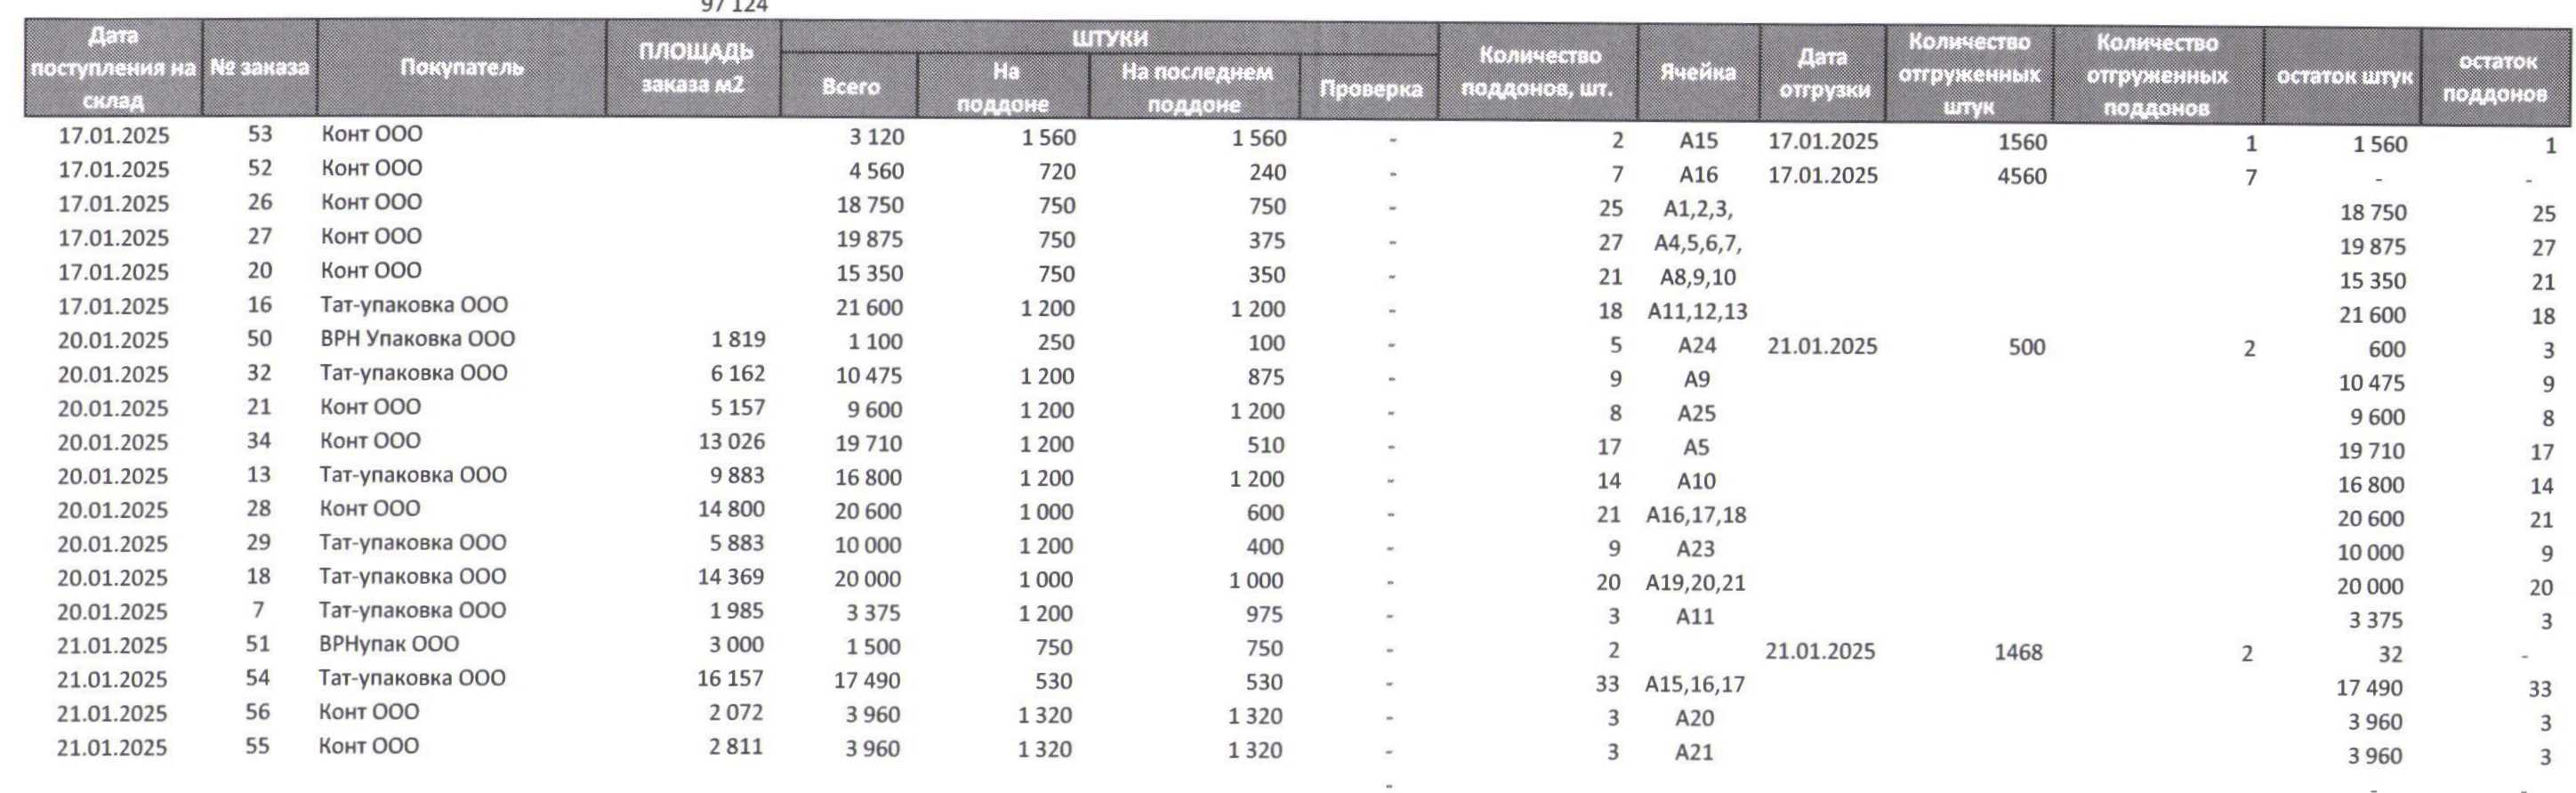
\includegraphics[width=\linewidth, height=0.94\textheight, angle=90, keepaspectratio]{Pics/f10.jpg}
\end{center}
\caption{Остатки готовой продукции на складе}
\label{pic:f10}
\end{figure}

\begin{figure}
\begin{center}
 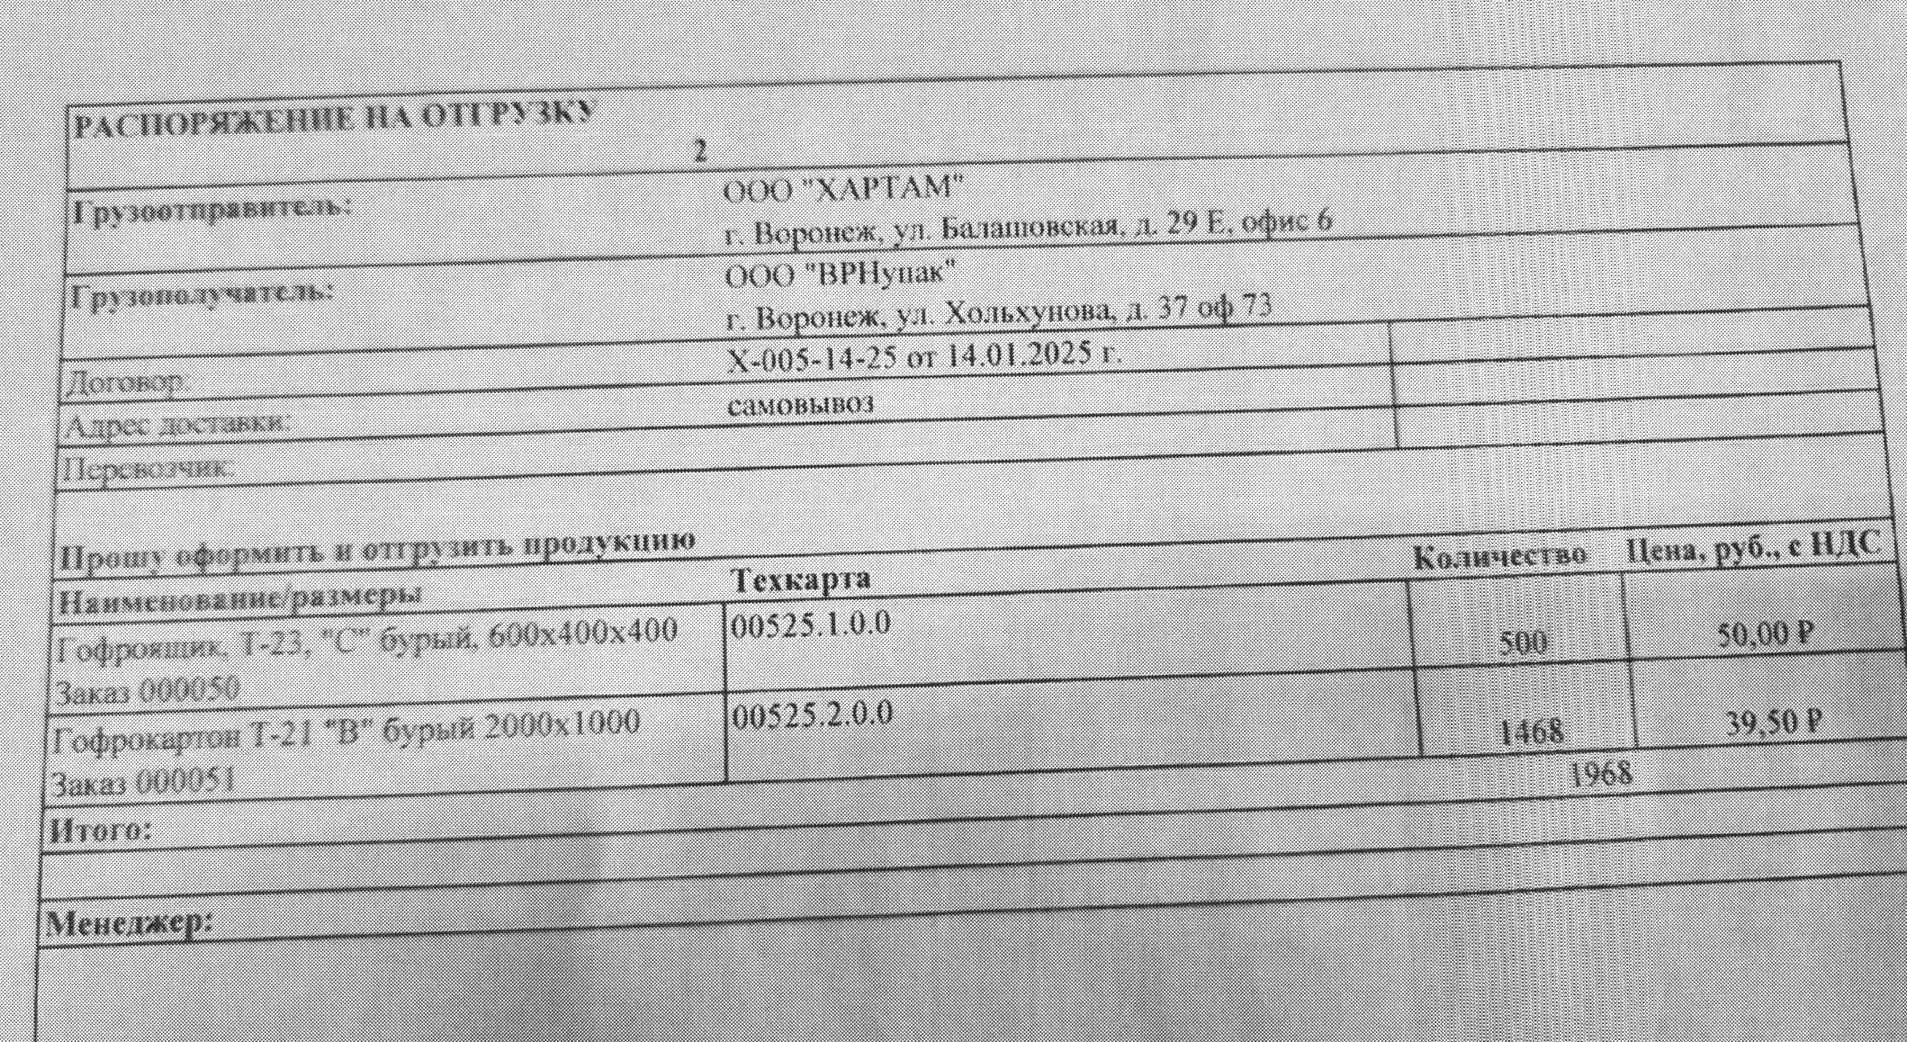
\includegraphics[width=\linewidth, height=0.94\textheight, keepaspectratio]{Pics/f11.jpg}
\end{center}
\caption{Распоряжение на отгрузку}
\label{pic:f11}
\end{figure}

\begin{figure}
\begin{center}
 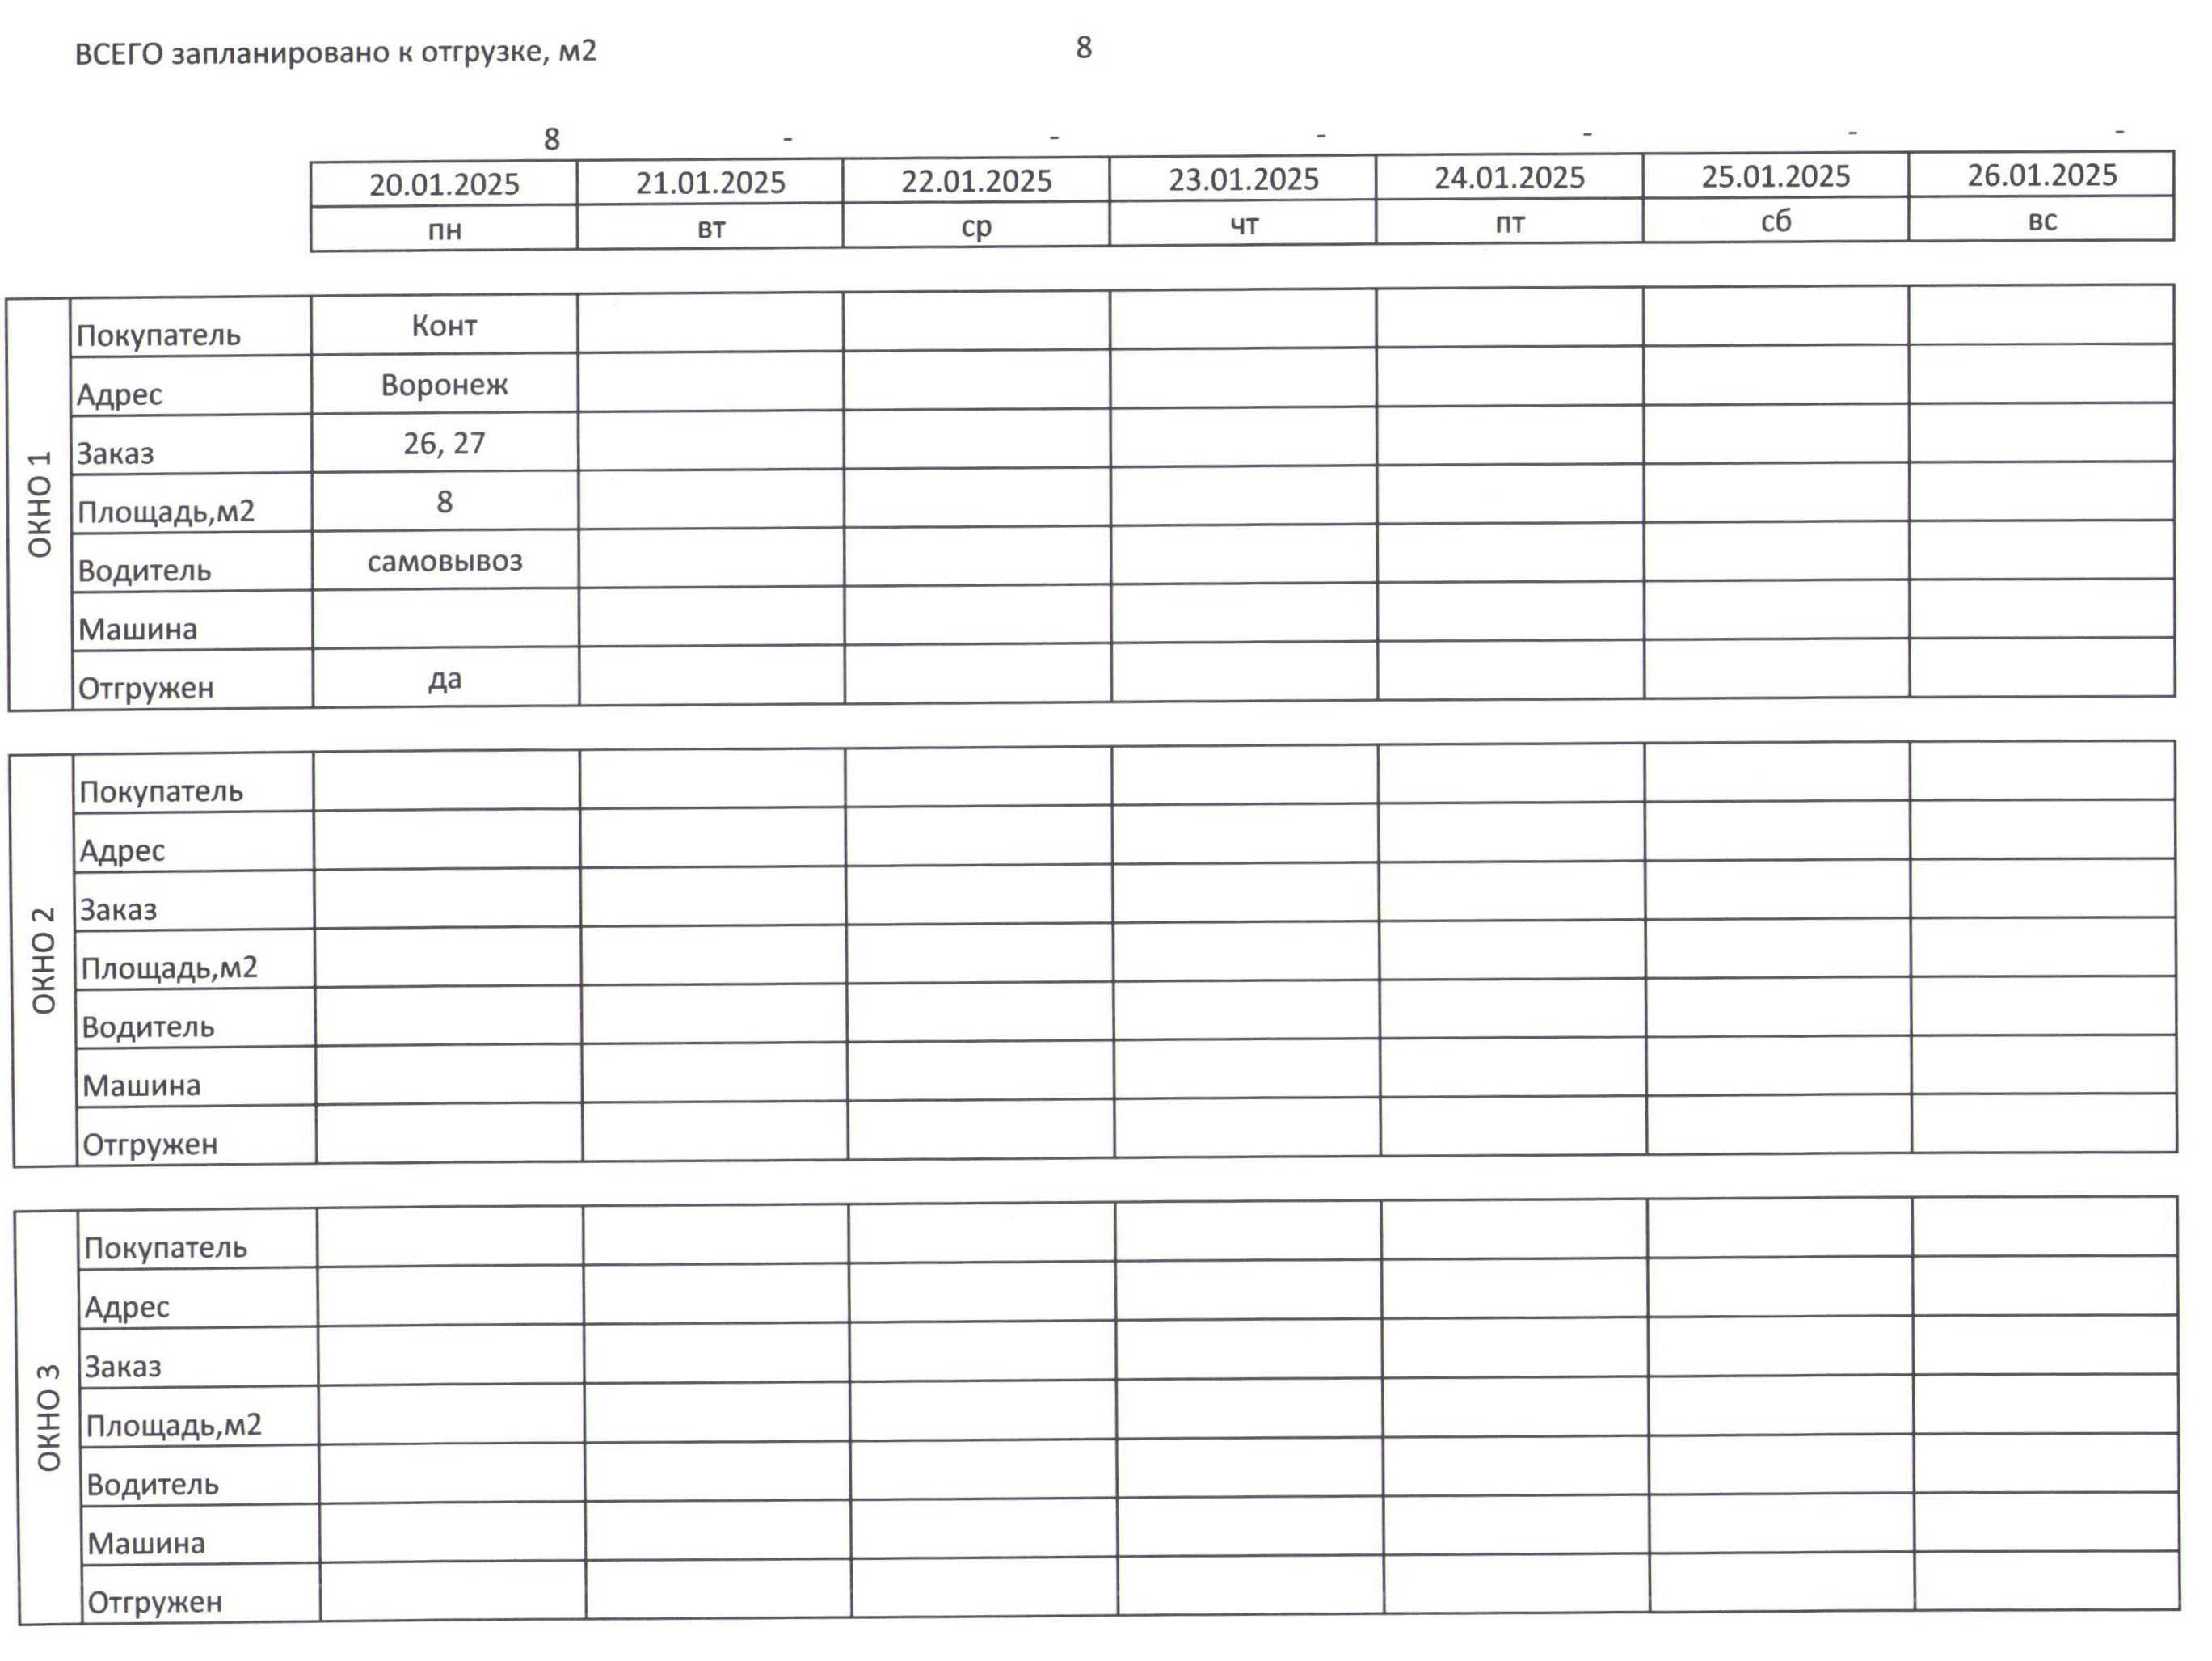
\includegraphics[width=\linewidth, height=0.94\textheight, keepaspectratio]{Pics/f14.jpg}
\end{center}
\caption{График отгрузки}
\label{pic:f14}
\end{figure}

